\documentclass{article}
\usepackage{amsmath}
\usepackage{amssymb}
\usepackage[top=25truemm,bottom=20truemm,left=20truemm,right=20truemm]{geometry}
\usepackage[dvipdfmx]{graphicx}
\usepackage{plext} % 日本語の各種設定
\begin{document}

\section*{課題研究一学期成果報告書}
今年度の課題研究ではFortranとCを使ってシンセサイザーを作り、演奏することを目標とした。\par
Fortranだけでは音声出力のライブラリが無いので、波形はFortranで生成・加工してCに送り、C側のPulseAudioを利用して音声出力を行う構造を採用した。大まかなフローチャートは以下の通り。\par
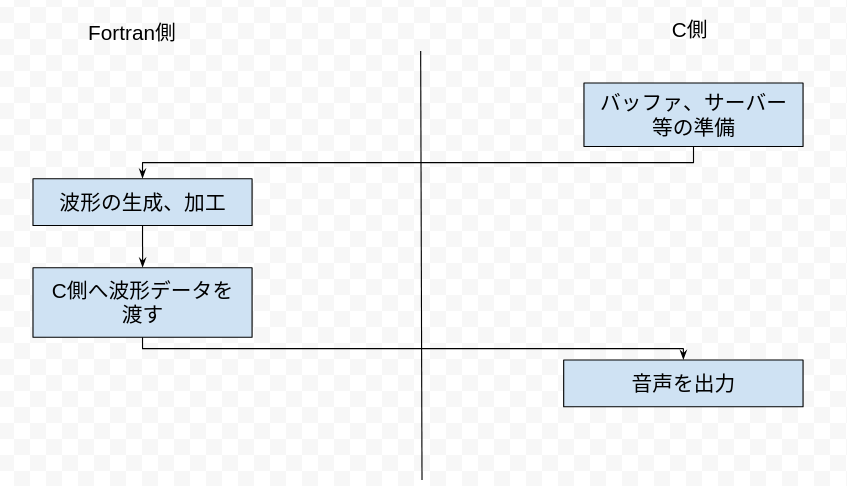
\includegraphics[width=175mm]{chart.png}
現在は、シンプルAPIを利用して一秒間正弦波を出力することに成功している。\par
今後の目標は
\begin{enumerate}
\item 非同期APIを使い、実用的なものにする
\item オシレータの種類を増やす
\item フィルタ、LFOを実装する
\item テキストファイルで演奏できるようにする $\leftarrow$ とても重要
\item raspberry pi pico、スピーカー、ゴムホースでトークボックスを作る
\item 最終目標として、完成したものを使って君が代を演奏する
\end{enumerate}

%% \subsection*{テーマ}
%% FortranとCを利用したシンセサイザー
%% \subsection*{成果}
%% \begin{enumerate}
%% \item PulseAudioシンプルAPIの利用
%% \item 一秒間の正弦波を音声出力
%% \end{enumerate}
%% \subsection*{今後の目標}
\end{document}
